\subsection{Sieve of Erathosthenes} \label{Sieve of Erastothenes}
The sieve of Eratosthenes, attributed to ancient Greek mathematician Eratosthenes of Cyrene, is an incredibly powerful algorithm which allows us to quickly exclude composite numbers from a list \citep[pp.332-335]{Horsley1772Sieve} by ``counting up''. In lieu of a strictly mathematical definition, the process can be best described by the following pseudocode \citep{WikiSieve}:
\begin{algorithm}
	\caption{Sieve of Eratosthenes}
	\KwIn{an intenger $n$, such that $n > 1$}
		 \textbf{Let} A be an array of boolean\footnotemark\ values, indexed by integers 2 to n, initially all set to true. \newline
		 	\For{$i = 2, 3, 4, ...,$ not exceeding $\sqrt{n}$}{
		 		
		 		\If{$A[i]$ is \textbf{true}}{
		 			\For{$j = i^2, i^2+i, i^2+2i,  i^2+3i,...,$ not exceeding $n$}{
		 				$A[j] := false$}
		 		}
	
		 		
		 	}
	
	\KwOut{all $i$ such that $A[i]$ is true.}	
	\caption{Sieve of Eratosthenes \citep{WikiSieve}}
	\label{alg:Sieve}
\end{algorithm}
\footnotetext{Boolean is a data type that can only either be true or false.}

In order to find all primes from 1 to 20 \textendash\ that is, $\pi(20)$ \textendash\ we begin by excluding all the multiples of the lowest prime, namely 2:

\textcircled{2}, 3, \cancel{4}, 5, \cancel{6}, 7, \cancel{8}, 9, \cancel{10}, 11, \cancel{12}, 13, \cancel{14}, 15, \cancel{16}, 17, \cancel{18}, 19, \cancel{20} \par
Followed by doing the same with the next lowest prime, 3: \par
2, \textcircled{3}, 5, 7, \cancel{9}, 11, 13, \cancel{15}, 17, 19\par
And repeating the process until all primes in the list have been found.
	
Thus, we have found the primes less than or equal to 20, namely $2, 3, 5, 7, 11, 13, 17, 19$ \textendash\ or in other words, $\pi(20) = 7$. While this ancient technique is quite powerful compared to the basic trial and error method discussed earlier, we are still forced to find each individual prime. Nevertheless, because it's just a repetitive task, we can have a computer run the algorithm (Appendix \ref{ap:Sieve}). In doing so, we find all primes less than $10^8$ before running into hardware limitations (Raw data in Appendix \ref{data:PrimesUpTo10^8}), and analyse our findings.
\begin{figure}[h]
\begin{tikzpicture}
\begin{axis}[
		xticklabels={0,0, $10^1$,$10^2$,$10^3$,$10^4$,$10^5$,$10^6$,$10^7$,$10^8$},
		ylabel = {$\pi(n)$},
		xlabel = {$n$}
]
	\addplot[color=blue, mark=square]
coordinates {
	(1,40)(2,25)(3,168)(4,1229)(5,9592)(6,78498)(7,664579)(8,5761455)
};
\end{axis}
\end{tikzpicture}
\caption{Distribution of primes}
\label{gr:ExpDistribution}
\end{figure}

Figure \ref{gr:ExpDistribution} seems to suggest some kind of exponential growth, however because the later values are so much larger than the first, the almost flat line we observe in the beginning hinders our analysis a little. Instead of plotting $\pi(n)$, we plot the frequency of primes \textendash\ that is $\frac{\pi(n)}{n}$ (Seen in figure \ref{gr:DistributionPrimes}). In looking for a ``relative'' of the exponential graph we hypothesised, we settle on $\frac{1}{\ln n}$, and present its graph in figure \ref{gr:1/lnx} for comparison.
	
\begin{figure} [h]
\begin{subfigure}{.50\textwidth}
	\centering
	\begin{tikzpicture}[scale=0.8]
	\begin{axis}[
	xticklabels={0,0, $10^1$,$10^2$,$10^3$,$10^4$,$10^5$,$10^6$,$10^7$,$10^8$},
	ylabel={$\frac{\pi(n)}{n}$},
	xlabel={$n$}
	];
	\addplot[color=blue, mark=square]
	coordinates {
		(1,0.40)(2,0.25)(3,0.168)(4,0.1229)(5,0.09592)(6,0.078498)(7,0.0664579)(8,0.05761455)
	};
	\end{axis}
	\end{tikzpicture}
\caption{Distribution of primes found utilising a Sieve of Eratosthenes. (Appendix \ref{ap:Sieve})}
\label{gr:DistributionPrimes}
\end{subfigure}%
\begin{subfigure}{.55\textwidth}
	\centering
	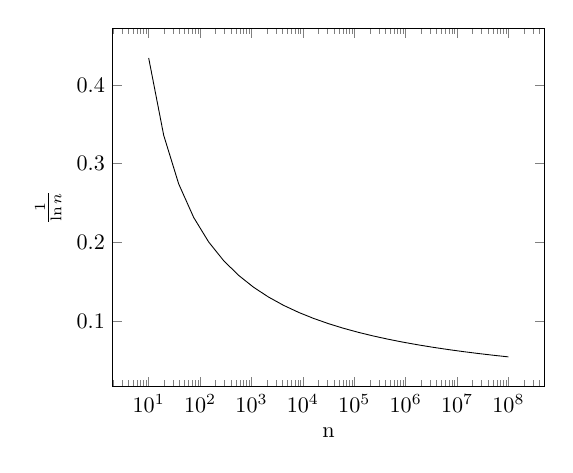
\begin{tikzpicture}[scale=0.8]
	\begin{axis}[
	xmode=log,
	ylabel={$\frac{1}{\ln n}$},
	xlabel={n},
	]
	\addplot[domain=10:100000000]{1/ln(x)};
	\end{axis}
	\end{tikzpicture}
\caption{$\frac{1}{\ln n}$ stipulated to follow the\\ same tendency as $\frac{\pi(n)}{n}$}
\label{gr:1/lnx}
\end{subfigure}
\caption{Comparison between the graphs for $\frac{\pi(n)}{n}$ and $\frac{1}{\ln n}$.}
\end{figure}


A comparison of the graphs suggests that their values converge for larger values of $n$. Thus we may present our first conjecture:
\begin{equation} \label{eq:FindingsFromSieve}
\begin{split}
	&\frac{\pi(n)}{n} \approx \frac{1}{\ln n} \quad \text{for large values of n} \\
	&\therefore \pi(n) \approx \frac{n}{\ln n} \quad \text{for large values of n}
\end{split}	
\end{equation}

Although the sieve itself could not be used to establish a significant distribution of primes for any $n$, equation \ref{eq:FindingsFromSieve} gives us the first stepping stone in our study for large values of $n$. Taking $10^{10}$, for instance, yields us $\frac{10^{10}}{\ln10^{10}} \approx 4.3 \cdot 10^8$, a really good estimate considering $\pi(10^{10}) \approx 4.5 \cdot 10^8$ \citep{CaldwellTableOfPi}.

Correspondingly, we are faced with two questions:
\begin{enumerate}
	\item Figure \ref{gr:DistributionPrimes} describes the behaviour up to $10^8$. Can this behaviour be expected to hold as $n$ becomes infinitely large?
	\item Does the frequency of prime numbers eventually reach zero?
\end{enumerate}

The former is in a way the very point of this study, whilst the latter requires a bit more information than a simple yes or no. As will be discussed further in this study, models for the distribution of primes are based on asymptotic analysis, which assume infinitely large values of $n$. This assumption is made possible by Euclid's Theorem, which proves the following:
\begin{Thm} \label{thm:EuclidsTheorem}
	There are infinitely many prime numbers.
\end{Thm}
Its proof follows an incredibly elegant logic \citep[pp. 147, 148]{ClawsonMathMysteries}.
\begin{Pro}
	(i) Suppose there is a finite number of primes $p_1$, $p_2$,$...$, $p_n$; \par
	(ii) Let $p\, |\, p \in$ $\{p_1, p_2, ..., p_n\}$; \par
	(iii) Let $P$ be a multiple of any combination of these primes plus one, that is, $P = p_1 p_2 ... p_n +1$. As such, $P$ is either prime or composite. \par
	(iii) If $P$ cannot be divided by $p$, then as per theorem \ref{thm:FTA}, it must itself be prime, and therefore (i) is incomplete.\par
	(iv) If $P$ is composite, it must therefore be divisible by $p$, which is impossible since $P \equiv 1 \, (\mod p)$; \par
\end{Pro}

The knowledge amassed so far allows us to move away from the idea of finding each individual prime and move towards prime counting functions.